% CVPR 2022 Paper Template
% based on the CVPR template provided by Ming-Ming Cheng (https://github.com/MCG-NKU/CVPR_Template)
% modified and extended by Stefan Roth (stefan.roth@NOSPAMtu-darmstadt.de)

\documentclass[10pt,twocolumn,letterpaper]{article}

\usepackage[pagenumbers]{cvpr} % To force page numbers, e.g. for an arXiv version

% Include other packages here, before hyperref.
\usepackage{graphicx}
\usepackage{amsmath}
\usepackage{amssymb}
\usepackage{booktabs}
\usepackage{paralist}

\usepackage[pagebackref,breaklinks,colorlinks]{hyperref}


% Support for easy cross-referencing
\usepackage[capitalize]{cleveref}
\crefname{section}{Sec.}{Secs.}
\Crefname{section}{Section}{Sections}
\Crefname{table}{Table}{Tables}
\crefname{table}{Tab.}{Tabs.}

\newcommand{\xhdr}[1]{\vspace{3pt}\noindent\textbf{#1}}
%%%%%%%%% PAPER ID  - PLEASE UPDATE
\def\cvprPaperID{*****} % *** Enter the CVPR Paper ID here
\def\confName{AI539}
\def\confYear{W2023}


\begin{document}

%%%%%%%%% TITLE - PLEASE UPDATE
\title{Friend or Foe? Detecting Adversaries in Hateful Subreddits}

\author{Bui, Vy \hspace{20pt} Chen, Chiu-Chun \hspace{20 pt} Helms, Derek \hspace{20 pt} Hickey, Dan \\
Oregon State University\\
{\tt\small \{buivy, chenchiu, helmsd, hickeyda\}@oregonstate.edu}
}
\maketitle

%%%%%%%%%%%%%%%%%%%%%%%%%%%%%%%%%%%%%%%%%%%%% ABSTRACT %%%%%%%%%%%%%%%%%%%%%%%%%%%%%%%%%%%%%%%%%%%%%
\begin{abstract}
   Recent work that seeks to make inferences about how individuals become radicalized in online environments samples users from hateful subreddits. However, these studies make the assumption that all users in these subreddits are aligned with the community's greater interests. In reality, many users enter hateful subreddits and employ ``counter-speech,'' which is language that refutes the hateful ideologies of the subreddits' core members. We take inspiration from the counter-speech detection and domain adaptation literature to build a model to detect such users in hateful subreddits. We then use this model to demonstrate how the quality of research on hateful subreddits can be improved by filtering adversaries of the subreddits out of samples.
\end{abstract}

%%%%%%%%%%%%%%%%%%%%%%%%%%%%%%%%%%%%%%%%%%%%% INTRODUCTION %%%%%%%%%%%%%%%%%%%%%%%%%%%%%%%%%%%%%%%%%%%%%
\section{Introduction}
%Discussing what it is that we are solving, why it is important, what problems are keeping this from being solved currently (detecting hate speech is a simpler task, but detecting counter hate provides more difficulty in terms of needing context), how does our approach solve this (discuss using context), what will determine success (not metric stats, but overall idea).

Online hate communities present a significant threat to the world, both online and offline. Numerous mass killings have been linked to perpetrators’ engagement in hateful online communities, and hate can make social media platforms less welcoming, especially for minority identity groups. Social media platforms, such as Reddit, have a unique role to play in this issue, as they make it easier than ever for hateful individuals to form communities and communicate with each other \cite{caiani2015transnationalization}. It is therefore essential to document the actions and dynamics of online hate groups to understand further how to moderate them and mitigate radicalization. Previous work in this domain has revealed important characteristics of hateful subreddits, such as the effect becoming active in a hateful subreddit has on users' language outside of the subreddits \cite{Schmitz2022}, or that members of hateful subreddits frequently attack newcomers, reducing their engagement in the hateful communities \cite{hickey2023reddit}. However, work of this nature that attempts to make inferences about hateful online users by sampling from hateful subreddits operates under the assumption that each member of each subreddit is genuinely hateful or prone to radicalization. While it is likely this is true for most users that post in hateful subreddits, this can nonetheless have an impact on studies like this. In some studies that sample from hateful subreddits, the quality of the samples can be improved by filtering out users who are not genuinely hateful. In other cases, knowing which users are not hateful can greatly affect the conclusions of a study. For example, in the study done by Hickey et al \footnote{This paper is not published yet, so the citation is fake. Just email Dan if you are curious about the details.} \cite{hickey2023reddit}, users of hateful subreddits were found to be hostile toward newcomers, and this hostility was associated with newcomers leaving the subreddits. The authors of this paper came to the conclusion that members of hateful subreddits were ineffective at recruiting new members through direct social interaction. However, if members of hateful subreddits are only hostile toward users who enter the community to criticize it, and those users are the ones who are being driven away, then that provides evidence that members of hateful subreddits are effective at driving away users they do not want to engage with their community. Furthermore, there is evidence subreddits benefit from being hostile toward outsiders who attack their community \cite{kumar2018community}.

In this report, we address and investigate this assumption by detecting ``adversaries'' in hateful subreddits -- users who express views that oppose ideologies of hate or the general views of core members of hateful subreddits. We pair datasets and methods from the counter-speech detection literature with the domain adaptation technique of self-training \cite{ruder2018strong} to detect such users. We test our model on a manually annotated set of 500 comments from hateful subreddits, then estimate the proportion of adversaries in hateful subreddits, as well as perform an analysis from Hickey et al. \cite{hickey2023reddit} with samples adjusted for adversaries to demonstrate the importance in adjusting for them in analyses.
Overall, we find that while results can be replicated from a prior counter-speech detection study, performance significantly drops for this new task and domain. Some strategies to adapt the task to our new domain result in dramatic improvements above the initial drop from the direct replication, though they do not get as high as the performance of the original study. Using our models, we demonstrate that adversaries are indeed prevalent in these subreddits, but not to the degree that they change the results of the analysis done by Hickey et al \cite{hickey2023reddit}. However, the performance of our method for detecting adversaries as well as the quality of our annotations are not high, so we suggest the results of this study be taken lightly and a more rigorous follow-up with an improved training set and annotation process, or more extensive domain adaptation experiments, be conducted.

%%%%%%%%%%%%%%%%%%%%%%%%%%%%%%%%%%%%%%%%%%%%% RELATED WORK %%%%%%%%%%%%%%%%%%%%%%%%%%%%%%%%%%%%%%%%%%%%%
\section{Related Work}
%Discussing the prior work of the original paper (what they aimed to do), how our work expands on what they started (new data + different overall goal), how our work is similar to others, what we based our code/setup off of (repo and paper), etc. This needs to compare and contrast our work and the previous papers.

\subsection{Online Hate Groups and Community Conflict}

Many previous works have sought to understand online hate and radicalization, which can inform moderation efforts of social media platforms. Causal modeling is commonly used in such studies as controlled experiments are difficult in social media settings \cite{founta2021survey}. Reddit users dramatically increase their usage of hateful language outside of hate groups when they become active in hate groups \cite{Schmitz2022}. Similarly, some studies have explored the impact of moderation of hateful communities, such as quarantines \cite{chandrasekharan2020quarantined} or bans \cite{horta2021platform} on the members of those communities, finding that hateful community membership is reduced with moderation efforts, but the users who stay may become more extreme. Other research measures the negative impact of hate speech on users' mental health \cite{saha2019prevalence}.
While the harms of hateful communities and language on social media are well-documented, there is still much work to be done on understanding why users become radicalized in the first place. Hickey et al. \cite{hickey2023reddit} attempt to help answer this question by documenting what factors of interaction in hateful communities cause users to keep posting in them.

While most subreddits are dedicated to discussions surrounding specific topics, including hate, it is not true that every user who posts in a given subreddit is a proponent of the topic of the subreddit. ``Brigading'' is a well-documented phenomenon, where an online community will attack another community in an organized manner, by either directing abusive speech toward the targeted community or exploiting popularity metrics (e.g. upvotes/downvotes) to reduce the visibility of views important to the targeted community \cite{graham2021sociomateriality, jhaver2018online}. One study that explored inter-community conflict on Reddit observed a ``colonizing'' effect of attacks on subreddits, where users from a community that attack a certain subreddit become more active in the attacked subreddit following the attack, while core users of the attacked community become less engaged. The authors observed that hostile responses toward such attacks often mitigated the colonizing effect of the attack \cite{kumar2018community}. Furthermore, another study of inter-subreddit conflict found subreddits similar to the ones studied in this report to be frequently involved in such conflicts \cite{datta2019extracting}.

\subsection{Counter-speech Detection}

Counter-speech is an approach to combating hate speech alternative to content moderation, wherein users of social media platforms reply to hateful language with arguments that refute or denounce such behavior \cite{mathew2019thou}. Counter-speech can take many forms, such as presenting facts to object to hate speech, responding to hate speech with humor, or even responding to hate speech with hostility. Mechanisms to promote counter-speech on social media are commonly recommended to platforms, as moderation efforts receive pushback from individuals who are concerned about excessive censorship \cite{mathew2020hate}. Counter-speech detection classifiers have been built using data from several domains, including YouTube \cite{mathew2019thou}, Twitter \cite{he2021racism, albanyan2022pinpointing}, and Reddit \cite{yu-etal-2022-hate, vidgen-etal-2021-introducing}. Some of these studies have also demonstrated how incorporating context into counter-speech datasets can improve performance \cite{albanyan2022pinpointing, yu-etal-2022-hate}. He et al. \cite{he2021racism} use their counter-speech classifier to find exposure to counter-speech decreases users' likelihood of becoming hateful on Twitter. To our knowledge, while counter-speech classifiers have been built using Reddit data, no extensive analyses of counter-speech in Reddit communities have been performed.

\subsection{Domain Adaptation in Natural Language Processing}
Most machine learning algorithms operate under the assumption that the test set is drawn from the same distribution as the training set \cite{ramponi2020neural}. Often, a model's performance will drop when applied to a different distribution, but in-distribution performance is also strongly correlated with out-of-distribution performance \cite{miller2021accuracy}. Common methods of domain adaptation involve changing aspects of the source model, such as the loss function or model structure. Other methods involve applying semi-supervised learning to unlabeled data \cite{ramponi2020neural}. Semi-supervised learning techniques include self-training, in which a model is trained on labeled data and used to predict classes on unlabeled data \cite{ruder2018strong}. The predictions above a certain confidence threshold are automatically labeled with their predicted class and removed from the set of unlabeled data. The high-confidence predictions are then used along with the original labeled data to train the model again. This process is repeated until there are no more high-confidence predictions. Another type of semi-supervised learning called tri-training uses three classifiers trained on bootstrapped labeled data. Unlabeled data points are added to the training set when all three models agree on the prediction. The process is repeated until no more data points can be added to the training set \cite{ruder2018strong}. We opt to employ self-training in this paper to improve performance under domain shift.

Label shift is another domain adaptation that can be considered for our problem. Black Box Shift Correction (BBSC) is a method to detect and quantify shifts between training and test set distributions, and apply corrections to the posterior probabilities in order to reflect original model performance onto a new class label distribution \cite{bbsc-lipton}. With fine-tuning being performed on the hate and counter hate speech data set originally proposed by Yu et al. \cite{yu-etal-2022-hate} and evaluation being performed on our new data collected from 25 different hateful subreddits, class labels have seen a shift as our domain has become hate-content specific. However, as the class distribution of our test set is similar to the class distribution of the data we trained our model on, we opted not to use this method.
%BBSC has been applied to our problem in order to account for this label shift, but results were unsuccessful in adapting to these changes. The shift correction weighted heavily to the majority class of non counter-hate speech, and as a result, all posterior probabilities were shifted to predict the majority. Results from this method were insufficient and are not reported in this paper.


%%%%%%%%%%%%%%%%%%%%%%%%%%%%%%%%%%%%%%%%%%%%% METHODOLOGY %%%%%%%%%%%%%%%%%%%%%%%%%%%%%%%%%%%%%%%%%%%%%
\begin{table*}[t]
  \centering
  \begin{tabular}{ l c c c c c }
    \toprule
    Method & Yu et al. F1 & Yu et al. ROC-AUC & New Domain F1 & New Domain ROC-AUC  \\
    \midrule
    Original Yu et al. Results \cite{yu-etal-2022-hate} & \textbf{0.53} & N/A & N/A & N/A \\
    Random Baseline & 0.32 & 0.5 & 0.26 & 0.5 \\
    Yu et al. Replication & 0.49 & 0.65 & 0.32 & 0.65 \\
    0\% $<$NULL$>$ Context Injection & 0.40 & 0.67 & 0.39 & 0.73 \\
    25\% $<$NULL$>$ Context Injection & 0.41 & 0.68 & \textbf{0.46} & \textbf{0.75} \\
    50\% $<$NULL$>$ Context Injection & 0.43 & 0.69 & 0.39 & 0.73 \\
    Target Only & 0.44 & \textbf{0.73} & 0.43 & 0.75 \\
    Target Only + Yu et al. Test Data & N/A & N/A & 0.39 & 0.74 \\
    Self-Training Method (Target Only) & 0.43  & 0.70  & 0.29 & 0.73 \\
    \bottomrule
  \end{tabular}
  \caption{Experimental results comparing Yu et al. test data vs new data performance. The $<$NULL$>$ context injection models and target only models were trained without the ``silver'' dataset from Yu et al.}
  \label{tab:example}
\end{table*}

\begin{figure}[t]
    \centering
    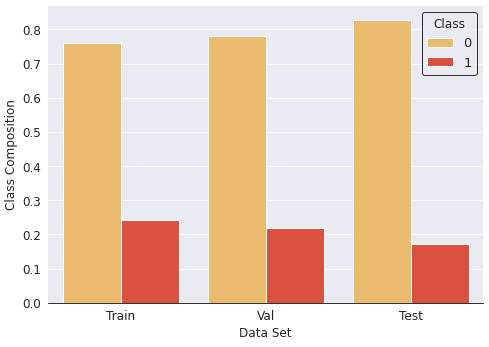
\includegraphics[scale=0.5]{class_distribution.png}
    \caption{Class composition per data split, with train and validation sets containing silver + gold from Yu et al. and test set containing observations from newly collected Subreddit data.}
    \label{fig:class dist}
\end{figure}


\section{Methodology}

\subsection{Replication of Yu et al.}
As a starting point for developing our own counter-speech detection model, we replicate a model built by Yu et al. \cite{yu-etal-2022-hate}. The authors used a dataset of 6,846 observations collected from Reddit by retrieving comments containing one or more hate words, which were then marked as the target variable, and their parent comments were marked as the context variable for that target \cite{yu-etal-2022-hate}. This creates the context/target pairs, which correlate to a ``post and reply'' general format to represent a conversation between two users. Annotation of these context/target pairs was completed through anonymizing and crowdsourcing the text to 674 different annotators, and was then split into two separate subsets: ``gold'' and ``silver'' data sets. The gold set consists of 4,751 pairs that had high agreeance among annotators (Krippendorf's $\alpha \geq 0.6$) while the silver set contains the 2,095 remaining pairs that had a lower agreement (Krippendorf's $\alpha < 0.6$). The Multi-Annotator Competence Estimation (MACE) score \cite{hovy-etal-2013-learning} was used to determine posts with high agreement \cite{yu-etal-2022-hate}, as annotations from individuals with low MACE scores were dropped to increase the agreement scores. The test set was derived only from examples in the gold dataset, while the silver dataset was used for training and validation in their highest-performing methods.

As a benchmark for replication, we refer to the highest F1 score reported by Yu et al. \cite{yu-etal-2022-hate} for counter-speech detection, which was 0.53. To achieve this score, the authors implemented pre-training a RoBERTa transformer \cite{liu2019roberta} on a stance detection dataset \cite{pougue2021debagreement} and fine-tuned the model with a combination of both gold and silver data sets, utilizing the combination of both context and target variables. We report results following this exact method, though we test other models that stray from this method, described in more detail in Section~\ref{sec:evaluation}.

While the authors built a multi-class classifier consisting of classes of ``hate,'' ``neutral,'' and ``counter-speech,''  our problem focuses mainly on the ability to replicate these methods only for the counter-speech class. This is because our domain is hateful subreddits rather than subreddits in general, and we want to detect users who explicitly state opposition to hateful ideologies. Furthermore, we make the assumption that there is a strong chance that users who use neutral language in hateful subreddits are hateful. Therefore, for all evaluations, we frame this as a binary classification problem.


\subsection{Evaluating Counter-hate Detection Models on Hateful Subreddit Data}\label{sec:evaluation}
To Expand on the work originally proposed by Yu et al. \cite{yu-etal-2022-hate}, we used a dataset of users' first posts in a set of 25 different hateful subreddits, spanning multiple targeted identity groups, collected by Hickey et al \cite{hickey2023reddit}. As these data are unlabeled, we manually labeled a small subset of 500 observations, sampled equally from each hateful subreddit. The posts were labeled to mirror the three classes from the Yu et al. data: hate (0), neutral (1), and counter-hate speech (2). Labelling was implemented by having each team member classify 50 of these observations in order to determine overall class agreement, and a single team member who is an expert in hateful subreddits moved forward with labeling the remaining observations. The observed Fleiss Kappa score among all annotators was 0.55, indicating moderate agreement. The distribution of labels between the original data and newly collected Subreddit data are nearly identical, with Figure~\ref{fig:class dist} representing the per class composition for each split. Utilizing this data to expand on the previous work, we evaluated multiple counter-hate detection models on the hateful subreddit data and reported values for both the F1 and ROC-AUC scores, with scores being evaluated based on the performance of the counter-hate speech class. In combination with this, the models were also evaluated on the original test data created by Yu et al. \cite{yu-etal-2022-hate} in order to compare model performance with the shift from general to hateful subreddit data for both metrics. 



%For evaluating performance on the new hateful subreddit data, a mixture of binary and multi-class tasks was performed and evaluated. For multi-class tasks, replication of Yu et al. \cite{yu-etal-2022-hate} was performed in order to determine if the modeling techniques utilized performed similarly to the original authors. For binary classification tasks, labels for both the original and new subreddits were grouped into two classes: non-counter-hate (0) and counter-hate (1), which are composed of hate + neutral and counter-hate speech, respectively. Binary classification tasks were trained and validated only on gold data sets due to higher agreeance among annotated labels and increased model performance. The purpose of the binary classification task was to determined if context has an impact on the ability to identify non counter-hate and counter hate speech in the target variable, which was tested through various methods. 

We evaluated multiple hypotheses of what could be done to maximize performance on our annotated test set. Firstly, we slightly alter the configuration of the model from what Yu et al. report achieved the best performance \cite{yu-etal-2022-hate}. As we noticed performance on the validation set was highest when only considering the ``gold'' dataset, we did not use the ``silver'' dataset for any of our further experiments. Then, we randomly replace the context training examples with $<$NULL$>$ tokens select thresholds to measure the difference in performance among models with missing context. The reasoning for this is that the PushShift API is missing some data \cite{gaffney2018caveat}, which means context examples will be unobtainable in certain cases. Indeed, 75\% of the examples in our annotated test set are missing context, with the average proportion per subreddit varying greatly (min. 16\%, max. 71\%, we double-checked the discrepancy between these values and the proportion in the test set and conclude we must have gotten very unlucky in sampling the test set). The second method involved training on target variables only, with no marker for missing context. This method was also re-implemented with the addition of the gold test set from Yu et al. \cite{yu-etal-2022-hate} during training, and evaluated only on the new subreddit data to determine the change in performance from increased training data sizes. Finally, self-training \cite{ruder2018strong} was employed using a set of 25,000 unlabeled Reddit posts, with 1,000 coming from each Subreddit. The confidence threshold for adding unlabeled predictions to the training set was 0.8.

In addition to the results for each model, we also report random baseline performance, wherein predicted labels were generated with an equal probability and the performance F1 score was calculated from those labels. The random label generation process was repeated 1,000 times and the mean F1 score was used as the final random baseline. Other random baselines were generated using a lower probability of labeling an example as counter-hate, but they were not as high as the equal probability case.

\subsection{Analysis of Adversaries in Hateful Subreddits}

To demonstrate the utility of our models, we apply our self-training model to the full unlabeled dataset collected by Hickey et al \cite{hickey2023reddit}. To provide greater context for this analysis, we will first summarize the previous work: First, all posts from 25 different hateful subreddits were collected using the Pushshift API \cite{baumgartner2020pushshift}. The first post of each user was taken from each subreddit, as well as the first reply from each of those posts if they received replies. The authors also recorded whether or not each user continued to post within other threads on the subreddit they initially posted in. Users who received replies to their first posts were matched with users who did not receive replies using causal inference methods, and the groups were compared. The authors found that users who received replies to their first posts in hateful subreddits were less likely to keep posting in them than users who did not receive replies. Furthermore, the authors matched hateful subreddits to non-hateful subreddits and found replies have the opposite effect in non-hateful subreddits. To investigate this discrepancy, the authors used the ``attack on commenter'' model from the Perspective API \cite{Jigsaw2017} and found that personal attacks are much more common in hateful subreddits compared to non-hateful ones, and attacks are strongly negatively associated with reduced engagement across all subreddits.

%To quantify this, we simply take the proportion of users labeled as adversaries based on their first posts, then adjust for the estimated rate of false positives and false negatives calculated from the test data. It should be noted this treats all users equally and does not adjust for activity levels, so adversaries may be measured as more prevalent than they would be perceived by a user on the Reddit platform.

There are two relevant problems that can be addressed using these data -- firstly, it is useful to know the overall prevalence of adversaries in hateful subreddits and which subreddits they are more common in. To do this, we measure the proportion of positive predictions from each users' first post in each hateful subreddit. It should be noted this treats all users equally and does not adjust for activity levels, so adversaries may be measured as more prevalent than they would be perceived by a user on the Reddit platform.

The next question that can be addressed is whether removing adversaries from the samples of users will change the results from Hickey et al. in any way. For the purpose of this report, we focus on the comparison between hateful and non-hateful subreddits in terms of the effect replies have on further engagement in the subreddits. As the samples consist of users who received replies matched directly with users who did not receive replies, any matched pair that contains an adversary is removed from the sample. In an ideal scenario, the matching process would be repeated after removing all adversaries from the samples, but for the sake of time, we simply remove matched pairs.

%%%%%%%%%%%%%%%%%%%%%%%%%%%%%%%%%%%%%%%%%%%%% RESULTS %%%%%%%%%%%%%%%%%%%%%%%%%%%%%%%%%%%%%%%%%%%%%
\section{Results}

\textbf{Results from Yu et al. could be replicated.} Table~\ref{tab:example} displays the results of all models we experimented with. We achieve an F1 score of 0.49 when replicating the method Yu et al. obtained their best results with. While this is not as high as the benchmark of 0.53, the result is still expected to happen by chance, as Yu et al. report a mean F1 of 0.5 and a standard deviation of 0.03 when training their model using a series of different random seeds \cite{yu-etal-2022-hate}. This indicates competence in our ability to train models, as we achieve performance comparable to the standard for published research using this training dataset. Additionally, it reinforces the validity of the research conducted by Yu et al.

\textbf{Domain adaptation techniques show mixed results.} When testing different levels of missing context in the training dataset, we found having context removed from some training examples helped improve performance on our labeled test set (Table~\ref{tab:example}). The best performance was acheived by randomly removing context from 25\% of the training examples (F1=0.46). However, training without any context was very close in performance (F1=0.43). Surprisingly, self-training results in the lowest performance on the labeled test set (F1=0.29), aside from the random baseline.


\begin{figure}
    \centering
    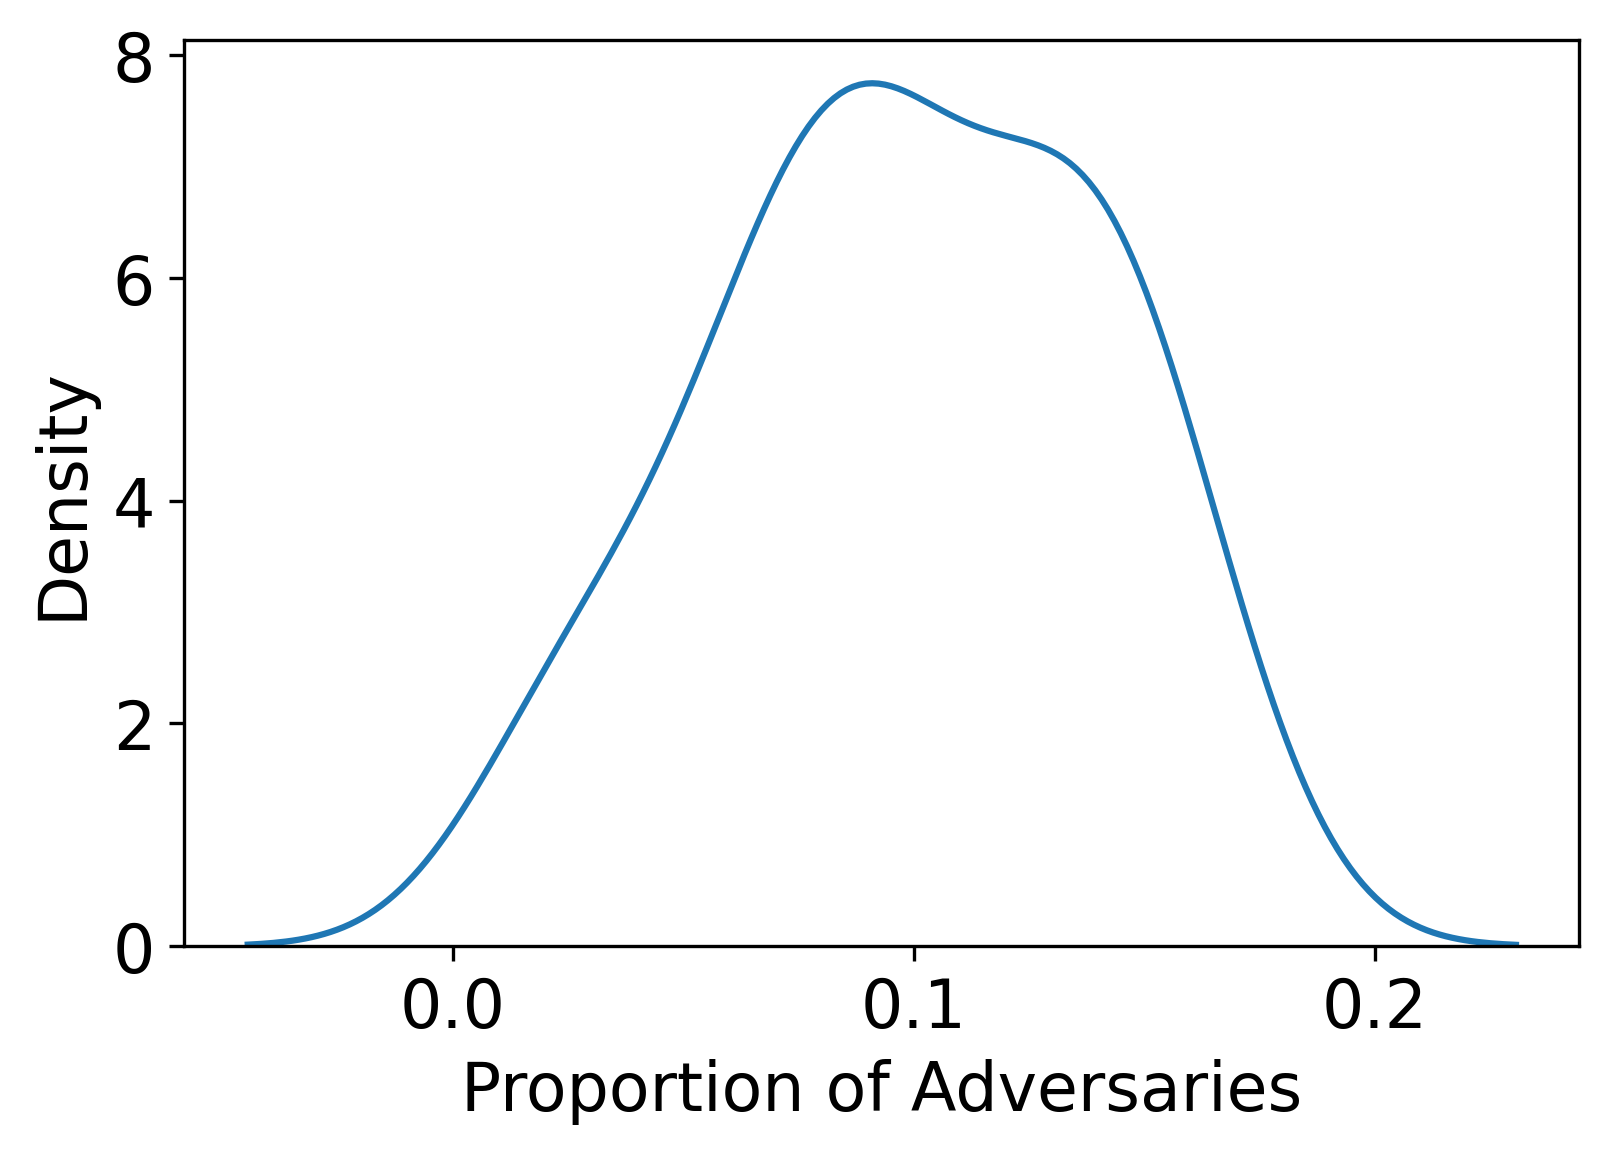
\includegraphics[width=0.9\columnwidth]{adversary_distribution.png}
    \caption{Distribution of proportions of adversaries in each hateful subreddit.}
    \label{fig:adversary_distribution}
\end{figure}

\textbf{Adversaries are prevalent in hateful subreddits.}

The distribution of proportions of adversaries in hateful subreddits is shown in Figure~\ref{fig:adversary_distribution}. The mean is 0.1 with a standard deviation of 0.04.


\begin{figure}
    \centering
    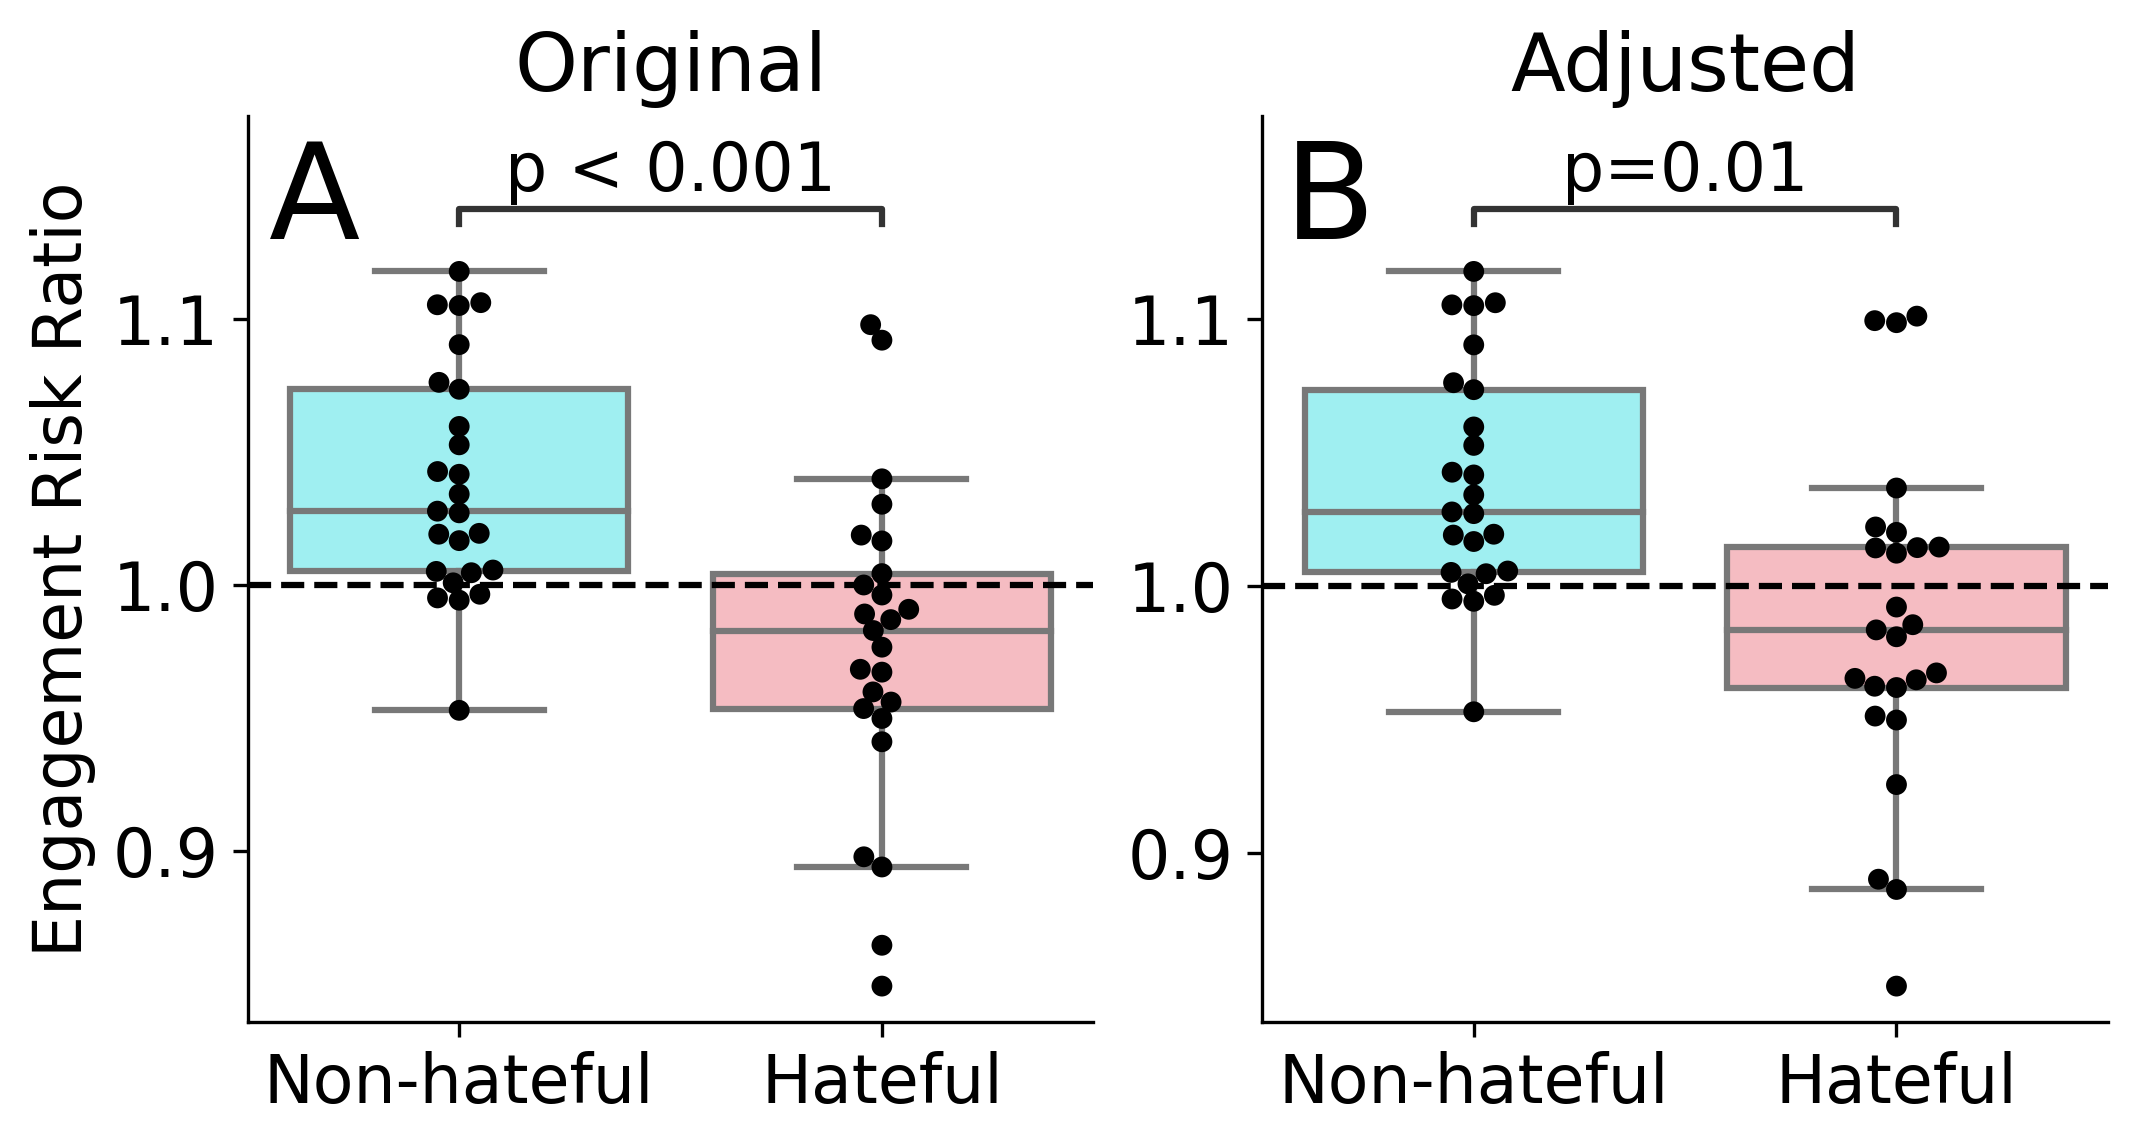
\includegraphics[width=0.9\columnwidth]{adjusted_adversaries.png}
    \caption{Results comparing the effects of replies on engagement in hateful subreddits using (A) the original sample from Hickey et al. and (B) the sample after removing matched pairs of users containing adversaries from hateful subreddits. An Engagement Risk Ratio greater than one indicates replies have a positive effect on engagement, while a ratio lower than one indicates replies have a negative effect.}
    \label{fig:adversary_comparison}
\end{figure}

\textbf{Results from Hickey et al. stay consistent when accounting for adversaries.}

Figure~\ref{fig:adversary_comparison} displays the results of the analysis of overall effects of replies in hateful subreddits before and after adjusting for adversaries. We find that the results are still statistically significant in favor of the original result from Hickey et al. \cite{hickey2023reddit}. However, the overall negative effect of replies is smaller after adjusting for adversaries.


%%%%%%%%%%%%%%%%%%%%%%%%%%%%%%%%%%%%%%%%%%%%% CONCLUSION %%%%%%%%%%%%%%%%%%%%%%%%%%%%%%%%%%%%%%%%%%%%%
\section{Conclusion}
In this study, we trained multiple counter-speech classification models to detect users in hateful subreddits who do not align with the general views of the community. We also demonstrated how the results of prior research can change when considering such users.

We attempted several strategies for improving performance under domain shift with mixed results overall. Some strategies, such as incorporating more training data, either in the form of the test set from the original training distribution, or weakly labeled data from the self-training method, performed worse than we expected. Furthermore, incorporating training data with low inter-annotator agreement also resulted in lower performance. While it is counter-intuitive that less data results in better predictions, it is possible that our model was overfitting to the distribution in the original domain when given more data from that distribution, so it generalized better to the new domain with less data. For the self-training method, it is possible that biases from the original distribution affected the labeling of data in the new distribution, and errors early on in the self-training process then propagated throughout the rest of the training set. However, more extensive validation of the parameters of the self-training process, such as training dataset size and confidence threshold, should be done before drawing any concrete conclusions. 

Lastly, while our classifiers are not extremely accurate, we nonetheless demonstrate how it is important for practitioners to consider how their samples of users from different hateful subreddits can include users that are not of interest to their research question. While we do not demonstrate that this changes the results of another research paper, it is still evident to us that this is a category of users that should be considered. We urge researchers studying hate groups or hate speech online to consider this possibility. Furthermore, we feel more confident in the conclusions made by Hickey et al. as we could not disprove them through this analysis.

\subsection*{Limitations and Future Directions}

\textbf{Annotation Quality.} Our whole test set was only annotated by one person, and for the portion that was annotated by multiple people, agreement among raters was moderate. Furthermore, capturing the nuances of the language used in specific hateful online communities requires extensive background knowledge and training. For these reasons, we caution that the final results of this report be taken lightly. An in-depth, expert-guided annotation process with disagreements discussed by annotators, as implemented by Vidgen et al. \cite{vidgen-etal-2021-introducing} would provide more clarity regarding the true performance of our model.

\textbf{Quality of training data.} While we chose to focus on data from Yu et al. \cite{yu-etal-2022-hate} to train our counter-hate model due to its similarity to our domain, we acknowledge the observed upper limit for overall performance on this dataset is low (F1=0.53). Notably, other researchers have achieved much higher F1 scores of 0.72 \cite{mathew2019thou} and 0.85 \cite{he2021racism} on data from YouTube and Twitter, respectively. It is possible that the data used to train these classifiers are of higher quality than the dataset we used, and the benefit of the increase in quality could overpower the detriment of a greater domain shift. Furthermore, both prior studies use data annotated by a small set of experts rather than annotations crowdsourced from Amazon Mechanical Turk (as was done by Yu et al \cite{yu-etal-2022-hate}). While we acknowledge the importance of reducing bias in annotations by sourcing them from a wide variety of people, there are also issues with annotations sourced from Mechanical Turk \cite{fort2011amazon}. Namely, we suspect the task of annotating counter-speech to be a difficult one that crowd workers have not been sufficiently trained for.

\textbf{More rigorous testing of domain adaptation strategies.} In this study, we evaluated the strategy of self-training to improve the performance of counter-speech classification under domain shift. Surprisingly, performance decreased when using this method. However, due to time constraints, this was the only method we tested, and there are many other methods that could be applied \cite{ramponi2020neural}. Even within the self-training method, there are hyperparameters we could have tuned given more time, such as the confidence threshold or max number of iterations. Furthermore, strategies such as tri-training have been demonstrated to outperform self-training \cite{ruder2018strong}. Performance would likely be improved by considering other domain adaptation methods.

\textbf{Impact of adversaries on hateful subreddits.} In this study, we observed how hateful individuals respond to their adversaries in hateful subreddits and how that can influence the staying power of the adversaries. However, we did not investigate the influence adversaries may have on the success of the hateful subreddits or the behavior of their members. This would be an important problem to investigate, as previous studies warn of the potential dangers of hateful individuals migrating to platforms where their views are challenged less frequently \cite{johnson2019hidden, copland2020reddit, horta2021platform}.




%%%%%%%%%%%%%%%%%%%%%%%%%%%%%%%%%%%%%%%%%%%%% REFERENCES %%%%%%%%%%%%%%%%%%%%%%%%%%%%%%%%%%%%%%%%%%%%%
{\small
\bibliographystyle{ieee_fullname}
\bibliography{egbib}
}

\end{document}
